
\documentclass[11pt,twocolumn,letterpaper]{article}


\usepackage{graphicx} % Required for inserting images
\usepackage[pagebackref]{hyperref}
\usepackage{comment}
\usepackage{multirow}
\usepackage{float}
\usepackage{titling}
\usepackage{amsmath}

\setlength{\droptitle}{-3em} 
\setlength{\topmargin}{0pt}
\setlength{\headheight}{0pt}
\setlength{\headsep}{0pt}
\setlength{\textheight}{\textheight}
\usepackage[margin=1in,footskip=.1in]{geometry}
\setlength{\footskip}{40pt} 



\title{COMP 433 Project Report}
\author{Jeremy Ouellette (ID: 40212872), Mazen Mahmoud (ID: 40175486)}
\date{Fall 2023}

\begin{document}

\maketitle

\section{Introduction}
% Introduce problem and sections
Label noise refers to inaccuracies or errors present in the assigned labels of a dataset used to train supervised machine learning models. In an ideal scenario, each data point (sample) should bear a correct label, guiding the model during training. However, real-world datasets often exhibit label noise, where certain data points carry incorrect or noisy labels. This poses a significant challenge for supervised learning models, as they depend on accurate labels to learn and to generalize patterns effectively. Label noise can originate from various sources, including human annotation errors and ambiguous instances that prove challenging to label. This issue is particularly pronounced in datasets designed to challenge humans, such as those from CAPTCHA systems, making them prone to label noise. 

However, despite the common practice of using deeper Convolutional Neural Networks (CNNs) to address complex tasks as is the case here, this approach falls short in handling label noise complexities. Indeed, only increasing model depth may worsen the problem by causing overfitting to noisy labels, reducing the model's ability to discern real patterns. 

This study aims to research the advantages of two specific techniques designed to increase resilience against label noise by comparing their outcomes with a baseline ResNet-18 CNN model. The report includes a comprehensive description of the noisy dataset in use, a thorough exploration of previous solutions through a literature study, an examination of the baseline model's characteristics and results, an in-depth analysis of each proposed technique's impact, and an overall comparison of the results.

\section{Dataset}
\begin{figure*}[!htb]
    \centering
    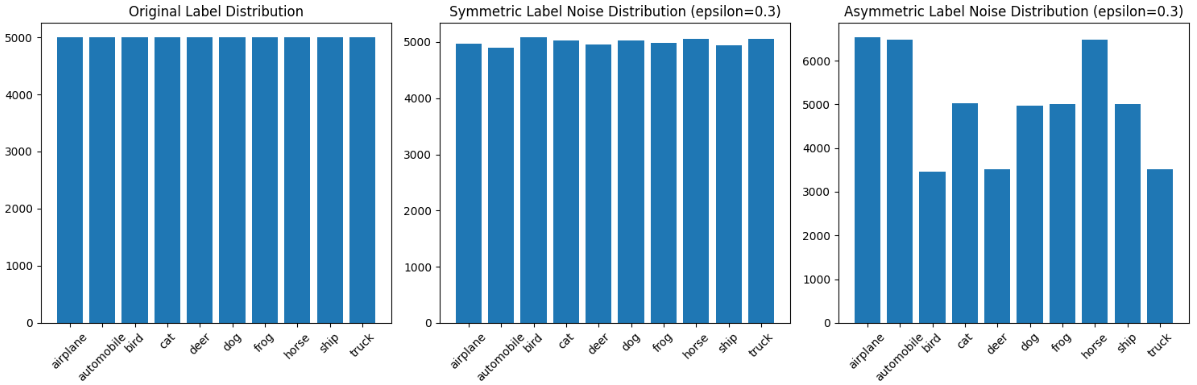
\includegraphics[width=1\linewidth]{dataset.png}
    \caption{Training set class distribution. The distribution is less uniform in the second and third graphs due to label noise.}
    \label{dataset}
\end{figure*}
The CIFAR-10 dataset comprises 60,000 32x32 color images distributed across 10 classes, with 6,000 images per class. It is divided into 50,000 training images and 10,000 test images. It includes the following classes: airplane, automobile, bird, cat, deer, dog, frog, horse, ship, and truck. These classes are mutually exclusive, with no overlap between automobiles and trucks. The "automobile" category encompasses sedans, SUVs, and similar vehicles, while the "truck" category includes only large trucks, excluding pickup trucks \cite{CIFAR10CIFAR100Datasets}.

\subsection{Introduction of Label Noise}

For this study, the CIFAR-10 dataset has been adapted to incorporate potentially noisy labels. The algorithms are designed to train on this modified dataset, taking into account two types of label noise:

\begin{itemize}
    \item \subsubsection*{Symmetric Label Noise}
    Symmetric label noise introduces uncertainty into the training data by flipping correct labels with a probability $\epsilon$. For instance, if there are 100 bird images in the training set and the noise level $\epsilon$, then $100(1 - \epsilon)$ of these images will retain the label "bird," while $100\epsilon$ will be randomly assigned a label different from "bird."
    \item \subsubsection*{Asymmetric Label Noise}
    Asymmetric label noise introduces label-flipping following predefined rules. As per the project requirements, the explicit rules for label flipping are as follows: "truck" should be flipped to "automobile," "bird" to "airplane," "deer" to "horse," "cat" to "dog," and "dog" to "cat." The determination of this flipping probability is tied to the asymmetric noise level $\epsilon$. To illustrate, if there are 100 bird images in the training data, $100(1 - \epsilon)$ of these should maintain the original "bird" label, while the remaining $100\epsilon$ bird images will undergo a label flip, changing their label to "airplane." 
\end{itemize}

Both symmetric and asymmetric label noise present challenges during training. On one side, symmetric noise introduces a stochastic noise as it mixes randomly the labels for all classes with all other classes. On the other side, asymmetric noise skews the learning in only one other way but more significantly. Figure \ref{dataset} summarizes the distribution of the training set from the original dataset and from its two derivatives.

\section{Literature Study}
To overcome the reduction in accuracy due to label noise, a large scope of strategies are available. These encompass the development of more robust architectures \cite{bahriDeepKNNNoisy2020} \cite{xiaAdaptiveGeneralModel2022}, the usage of specialized loss functions \cite{englessonGeneralizedJensenShannonDivergence2021} \cite{maNormalizedLossFunctions2020} \cite{xuL_DMIInformationtheoreticNoiserobust2019}, selective sampling techniques \cite{songLearningNoisyLabels2022} \cite{chenSamplePriorGuided2022}, and others \cite{songLearningNoisyLabels2022}. The next subsection will do a brief overview of the three main strategies that were researched in this work.

\subsection{Main Strategies}

\subsubsection{Noise Resilient Architectures}

To avoid the burden of dealing with noisy labels in the first place, it is possible to use unsupervised machine learning techniques that do not require any labels during training. Popular unsupervised models are k-means clustering \cite{bahriDeepKNNNoisy2020} and probability density estimation \cite{xiaAdaptiveGeneralModel2022}, where the former does not allow samples to be members of more than one category, but the latter does. These strategies use the insight that samples like images that have similar features are likely to be in the same category, and all that is needed is to know beforehand the number of categories. However, these techniques are not fit to be trained directly on CIFAR-10 as each image, should be embedded first into a feature vector created with the help of a trained CNN model (or any other model capable of this task) where its last classification layer is removed \cite{sejutiHybridCNNKNN2023a}.

Semi-supervised machine learning techniques are also an interesting alternative implemented in various works \cite{tongxiaoLearningMassiveNoisy2015}. They allow the model to be trained on a small sample of correctly labeled data and then on the rest of the data by making an abstraction of their noisy labels. This requirement could, however, not be met in this report as the noise is applied to the entire CIFAR-10 dataset.

Another promising approach exploited recently is to leverage early learning. Indeed, in the first epochs, DL models tend to learn features that generalize better compared to the learning done in the last epochs which tend to overfit more to the noise. Recent SOTA architectures leverage this knowledge to increase their robustness against noise \cite{liuEarlyLearningRegularizationPrevents2020} \cite{baiUnderstandingImprovingEarly2021}.

\subsubsection{Robust Loss Function:}
Choosing the right loss functions is crucial in making machine learning (ML) models strong against noise. In the last years, there has been a rise in interest in normalized loss functions as it was proven to increase robustness if a majority of labels in a class are correctly labeled \cite{englessonGeneralizedJensenShannonDivergence2021} \cite{maNormalizedLossFunctions2020}. However, this effort to boost robustness sometimes leads to a new problem called underfitting. Even though well-known loss functions like cross-entropy and focal loss become resilient with normalization, it doesn't always make the models more accurate overall. In fact, normalized cross-entropy and normalized focal loss usually perform even worse than their regular versions \cite{maNormalizedLossFunctions2020}. Because of this interest in hybrid loss functions merging both traditional, fast-converging loss and normalized more resilient loss rose \cite{wangSymmetricCrossEntropy2019} \cite{maNormalizedLossFunctions2020}. One popular example is `NCEandRCE`, combining Normalized Cross-Entropy (NCE) and Reverse Cross-Entropy (RCE) where the final output is a linear combination of both \cite{maNormalizedLossFunctions2020}. Another interesting loss is called 'Bootstrapping' where prior knowledge about the noise ratio is used in the loss function to overfit less to noise \cite{GJSLossesPy}.


\subsubsection{Sample Selection}
\begin{figure}[!h]
    \centering
    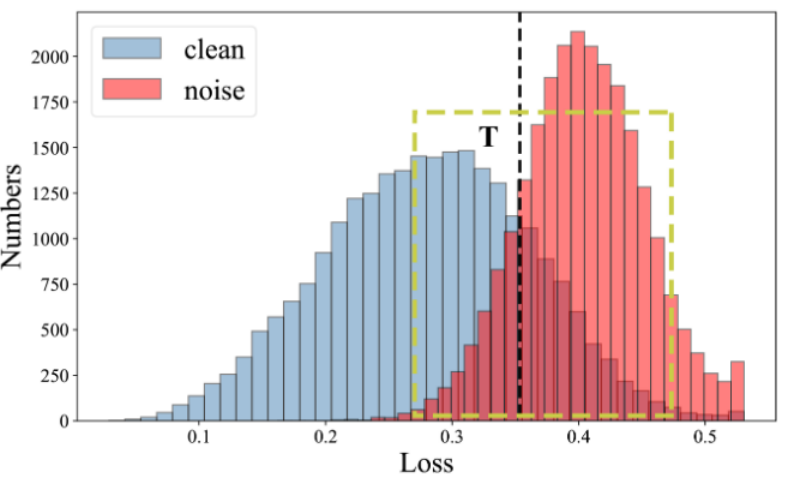
\includegraphics[width=1\linewidth]{distribution1.png}
    \caption{The distribution of losses for both clean and noisy samples in CIFAR-100, where 50\% of the noise is symmetrically introduced. Extracted from PGDF paper \cite{chenSamplePriorGuided2022}.}
    \label{fig:distribution1l}
\end{figure}

Sample selection is concerned with locating noisy samples during training and reducing their impact. Common techniques follow:

\begin{itemize}
    \item \textbf{Outlier Detection \cite{songRobustLearningSelfTransition2021} \cite{chenSamplePriorGuided2022}:}
    \begin{itemize}
        \item Identify samples deviating significantly in feature space.
        \item Utilize statistical measures or machine learning models for outlier detection.
        \item Exclude or down-weight identified outliers during training.
        \item See Figure \ref{fig:distribution1l}
    \end{itemize}
    
    \item \textbf{Consistency Checks:}
    \begin{itemize}
        \item Train multiple models on different data subsets.
        \item Evaluate the consistency of predictions across models for each sample.
        \item Consider samples with inconsistent predictions as potentially noisy.
    \end{itemize}
    
    \item \textbf{Confidence Estimation: \cite{xiaAdaptiveGeneralModel2022}}
    \begin{itemize}
        \item Utilize models providing confidence estimates for predictions.
        \item Set a threshold on prediction confidence to identify potentially noisy samples.
    \end{itemize}
    
    \item \textbf{Transfer Learning \cite{leeCleanNetTransferLearning2018}:}
    \begin{itemize}
        \item Leverage pre-trained models on clean data to identify noisy samples.
        \item Fine-tune the model on the new dataset, excluding or down-weighting noisy samples.
    \end{itemize}
\end{itemize}

\section{ResNet18 Baseline}
ResNet, introduced in 2015, stands out as a simple yet powerful baseline for its scalable architecture and innovative skip connections \cite{heDeepResidualLearning2015}. This addresses challenges in training very deep models, a limitation faced by earlier architectures like VGG \cite{simonyanVeryDeepConvolutional2015} and GoogLeNet \cite{szegedyInceptionv4InceptionResNetImpact2017}. Its impact is evident in subsequent models such as ResNeXt \cite{xieAggregatedResidualTransformations2017} and EfficientNet \cite{tanEfficientNetRethinkingModel2020}, all adopting the concept of skip connections for improved scalability and performance. Even in its lightweight form, ResNet18 maintains simplicity while striking a balance between model complexity and efficiency, making ResNet a foundational choice in modern computer vision tasks. The ResNet block is illustrated in Figure \ref{fig:resnetBlock} in the appendix. 

\subsubsection*{Hyperparameter Search}

We conducted a hyperparameter search for optimal model performance, experimenting with batch sizes of 64, 128, 256, and 512. Learning rates were adjusted accordingly, starting at 0.001 for a batch size of 64 and scaling for larger batches (e.g., 0.002 for 128, 0.004 for 256). Surprisingly, a learning rate of 0.006 performed better for a batch size of 512, compensating for fewer weight updates in larger batches. This scaling prevents an increase in epochs needed for convergence. Optimal results were observed at 10 epochs, as ResNet18 with standard Categorical Cross Entropy (CE) loss showed signs of overfitting beyond this point. We chose the ADAM optimizer due to faster convergence than SGD. Despite testing ResNet34, its longer training and inference times, driven by a larger number of weights, made it impractical within our time constraint for model training.

For a balanced approach considering computational efficiency and model accuracy, we selected a batch size of 256 and a learning rate of 0.004. This choice strikes a compromise between computational cost, training speed, and achieving satisfactory accuracy. Results in the appendix showcase an alternative configuration with a learning rate of 0.001 and a batch size of 64 \ref{tab:mergedAccuracyAdditional}. While it exhibits higher training accuracy, the improvement in test accuracy is limited. Hence, the chosen configuration with a batch size of 256 and a learning rate of 0.004 stands as a practical compromise, ensuring both accuracy and fast training time.

\subsection*{Result Analysis}
The outcomes, detailed in Table \ref{tab:mergedAccuracy} and summarized in Figure \ref{fig:BaselineResults}, showcase a notable decline in test accuracy as label noise intensifies, dropping from 78.13\% to 10.44\% in symmetric conditions (0.1 to 0.9). A similar pattern is evident in asymmetric noise conditions. Intriguingly, results for asymmetric noise exhibit more promise, with test accuracy at the highest noise level surpassing expectations. These findings highlight the inherent difficulty for our baseline model to sustain accuracy in the face of increased label noise, underscoring the necessity to explore more advanced solutions. On a positive note, the model demonstrates swift inference times, fluctuating between 0.0035 and 0.005 seconds, while training time for each noise level records around 200 seconds, utilizing a 32-bit precision V100 GPU on Google Colab. An alternative hyperparameter configuration is shown in the appendix \ref{tab:mergedAccuracyAdditional}.

\begin{table}[h]
\centering
\begin{tabular}{|c|c|c|c|c|}
\hline
\textbf{\(\epsilon\)} & \multicolumn{2}{c|}{\textbf{Symmetric}} & \multicolumn{2}{c|}{\textbf{Asymmetric}} \\
\cline{2-5}
 & \textbf{Train} & \textbf{Test} & \textbf{Train} & \textbf{Test} \\
\hline
0.1 & 63.77 & 76.92 & 70.95 & 77.32 \\
\hline
0.3 & 44.38 & 71.31 & 64.45 & 73.50 \\
\hline
0.5 & 29.40 & 66.80 & 59.64 & 59.57 \\
\hline
0.8 & 10.96 & 21.89 & 67.65 & 46.08 \\
\hline
0.9 & 10.00 & 9.83 & 71.54 & 46.73 \\
\hline
\end{tabular}
\caption{Baseline Train and Test Accuracies for Symmetric and Asymmetric Noise (batch\_size = 256 and learning\_rate = 0.004) and the output in percentage.}
\label{tab:mergedAccuracy}
\end{table}

\begin{figure}[ht]
    \centering
    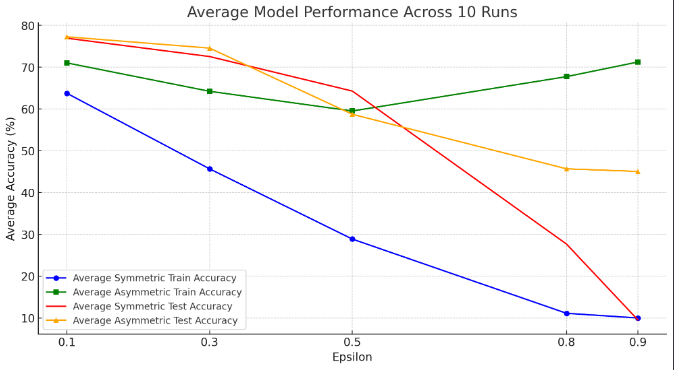
\includegraphics[width=1\linewidth, trim={0 0 10pt 0}, clip]{baselineResults.png}
    \caption{Baseline ResNet18 Results.}
    \label{fig:BaselineResults}
\end{figure}

\section{Proposed Solution Overview}
\subsection{ResNet18 with SCE Loss}

The first strategy we implemented to counter accuracy reduction related to label noise is to replace the categorical Cross-Entropy (CE) function with the Symmetric Cross-Entropy Loss (SCE Loss).

\subsubsection*{SCELoss: Symmetric Cross-Entropy Loss}

The \texttt{SCE Loss} is a custom loss function designed to handle label noise in classification tasks. Unlike some methods that use normalized loss functions and risk underfitting, SCE avoids underfitting by not using normalization at all. Instead, it supplements the traditional Cross Entropy Loss (CE) with Reverse Cross Entropy Loss (RCE). This balanced approach aims to enhance robustness without sacrificing accurate model predictions in the presence of label noise. This strategy was originally introduced in this work \cite{wangSymmetricCrossEntropy2019} under the name SL. We were inspired to implement this solution due to its ability to extract less noisy features from CIFAR-10 as showcased in Figure \ref{fig:SL} where the clusters in (b) are way purer compared to (a). 

\begin{figure}[ht]
    \centering
    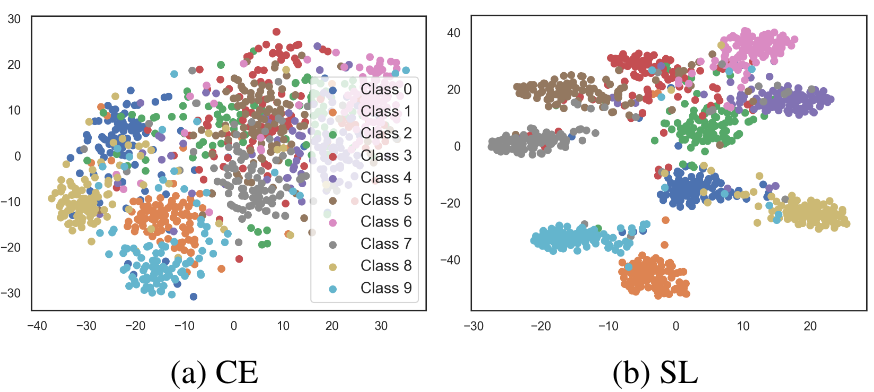
\includegraphics[width=1\linewidth]{SCESeparation.png}
    \caption{Representations acquired by CE and SL on the CIFAR-10 dataset containing 60\% symmetric noisy labels. Figure extracted from the SL paper \cite{wangSymmetricCrossEntropy2019}}
    \label{fig:SL}
\end{figure}
\subsubsection*{Cross-Entropy Loss (CE)}

Traditional Cross-Entropy Loss is a widely used metric in classification tasks. It quantifies the disparity between the predicted probability distribution and the true distribution of the labels. Mathematically, CE is defined as the negative log-likelihood of the true class:

\[
\text{CE}(p, q) = -\sum_{i} p_i \cdot \log(q_i)
\]

Here, \( p \) represents the true probability distribution (one-hot encoded labels), and \( q \) denotes the predicted probability distribution generated by the model.

\subsubsection*{Reverse Cross-Entropy Loss (RCE)}

Reverse Cross-Entropy Loss is introduced as a modification to traditional CE loss to enhance the model's robustness to label noise. RCE reverses the role of the true and predicted distributions, emphasizing correct predictions for instances where the true class probability is high:

\[
\text{RCE}(p, q) = -\sum_{i} q_i \cdot \log(p_i)
\]

Here, \( p \) represents the predicted probability distribution, and \( q \) is the true probability distribution (one-hot encoded labels).

\subsubsection*{Merging CE and RCE}

The \texttt{SCELoss} combines traditional CE and RCE, introducing a weighted sum of both losses. The parameters \( \alpha \) and \( \beta \) control the contribution of each term. The final SCE loss is given by:

\[
\text{SCELoss} = \alpha \cdot \text{CE} + \beta \cdot \text{RCE}
\]

The motivation behind SCE is to leverage the strengths of both CE and RCE to effectively handle label noise. CE focuses on correctly classifying instances where the predicted probability is high, while RCE emphasizes correct predictions when the true class probability is high.

The additional \texttt{clamp} operations applied to the predicted probabilities and one-hot encoded labels in the code are used to prevent numerical instability, ensuring numerical robustness during computation.

\subsubsection*{Hyperparameter Search}

We used the same batch size and learning rate combinations as in the baseline, but as the SCE loss converged a bit slower than CE with ADAM, we increased the number of weight updates by setting the batch size to 64 and the learning rate to 0.001. For \( \alpha \) and \( \beta \), both were set to 1 as recommended in the SCE paper, meaning equal weights for CE and RCE in the final output. As there were no signs of SCE overfitting to noise after 10 epochs, we extended training to 15 epochs. While a higher number could have been beneficial, resource constraints limited the training time.

\subsubsection*{Result Analysis}
ResNet18+SCE results are showcased in Table \ref{tab:mergedAccuracySCE} and Figure \ref{fig:SCEResults}. For all symmetric noise levels, the improvements in test accuracy in percentage points are as follows: 1.63, 4.66, 5.65, 11.71, and -0.59. It is clear that as noise increases, improvements over the baseline become more pronounced. For asymmetric noise levels, the changes are relatively small: 1.3, 4.7, -0.79, -0.55, -1.31. The inference time is  approximately the same as the baseline and the training time for each noise level was around 370 seconds on Colab's V100 with 32-bit precision.

\begin{table}[h]
\centering
\begin{tabular}{|c|c|c|c|c|}
\hline
\textbf{\(\epsilon\)} & \multicolumn{2}{c|}{\textbf{Symmetric}} & \multicolumn{2}{c|}{\textbf{Asymmetric}} \\
\cline{2-5}
 & \textbf{Train} & \textbf{Test} & \textbf{Train} & \textbf{Test} \\
\hline
0.1 & 77.57 & 78.55 & 83.09 & 78.62 \\
\hline
0.3 & 57.84 & 75.97 & 74.42 & 78.20 \\
\hline
0.5 & 39.08 & 72.45 & 67.94 & 58.78 \\
\hline
0.8 & 12.69 & 33.60 & 78.88 & 45.53 \\
\hline
0.9 & 9.97 & 9.24 & 83.40 & 45.42 \\
\hline
\end{tabular}
\caption{ResNet18+SCE Train and Test Accuracies for Symmetric and Asymmetric Noise (batch\_size = 64 and learning\_rate = 0.001) and the output in percentage.}
\label{tab:mergedAccuracySCE}
\end{table}

\begin{figure}[ht]
    \centering
    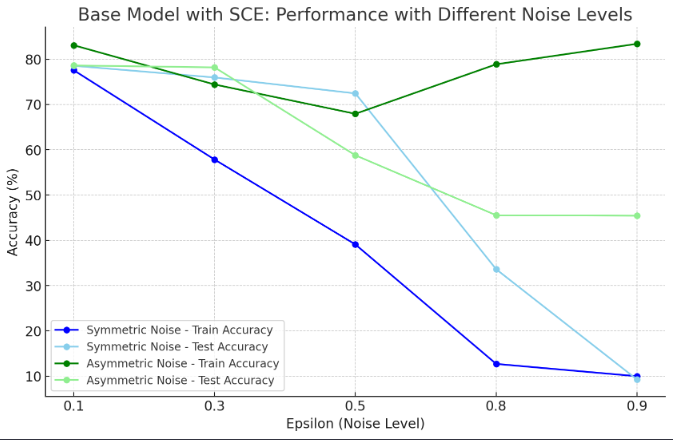
\includegraphics[width=1\linewidth, trim={0 10pt 0 0}, clip]{SCEResults.png}
    \caption{RestNet18 with SCE Loss Results}
    \label{fig:SCEResults}
\end{figure}

\subsubsection*{Additional Motivation}
Our decision to implement the SCE loss comes from extensive testing of other alternatives. We implemented and trained with L\_DMI, NCE+RCE, Normalized CE, Normalized RCE, Generalized CE, Mean Absolute Error (MAE), label smoothing-based loss, and bootstrapping-based loss. In all of these losses, with no exception, we experienced underfitting with accuracy often under 30\% on the training set for a symmetric noise level of 0.1 and 10 epochs. We tested each of them with ResNet18, ResNet34, EfficientNet-B0, EfficientNet-B1, and EfficientNet-B3 with no improvement for any of them. We believe that as most of these methods converge much slower compared to CE, they would have benefited from way longer training (\>100 epochs). Indeed, even with SCE not using any normalization hindering convergence speed, 15 epochs were still a serious limitation, as can be seen in Figure \ref{fig:convergence}. For this reason, the SCE loss is, to our knowledge, the best balance between training time, inference time, and test accuracy.

\begin{figure}
    \centering
    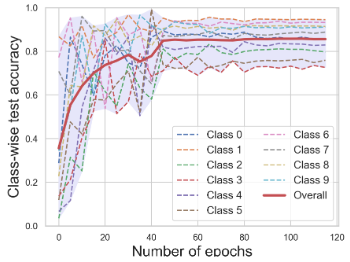
\includegraphics[width=1\linewidth]{convergence.png}
    \caption{ResNet34 accuracy wrt. epochs on CIFAR-10 (40\% symmetric label noise). Extracted from the SCE paper \cite{wangSymmetricCrossEntropy2019}.}
    \label{fig:convergence}
\end{figure}


\subsection{EfficientNet-B3 with SCE Loss and Transfer Learning}


The second strategy to increase resilience against label noise implemented for this work was to replace resnet18 with a pre-trained EfficientNet-B3 with the Symmetric Cross-Entropy Loss (SCELoss).

\subsubsection*{EfficientNet-B3 Characteristics}

EfficientNet-B3 was developed using Neural Architecture Search (NAS), an automated method for designing neural network structures. NAS explores a vast space of possible architectures to find an optimal configuration for a specific task. In contrast, ResNet18 is a manually designed architecture with predefined layer configurations. While the ResNet family is a well-established architecture, the EfficientNet family often outperforms it in terms of performance and model size efficiency as showcased in this figure \ref{fig:efficientNet}. On top of its better parameter efficiency, EfficientNet-B3 was chosen as it featured a similar number of parameters compared to ResNet18 (slightly lower) as it seemed like a fairer comparison with the baseline, and as it is available pre-trained on the ImageNet dataset.   

\subsubsection*{Motivation}
The main motivation behind this decision comes from the influence of recent works like ELR \cite{liuEarlyLearningRegularizationPrevents2020} demonstrating that only the early part of the training truly helps the models to generalize well to unseen data and after a moment the learning will mostly train the model to overfit to the noise. Therefore, based on this insight, it makes a lot of sense to use a pre-trained model and fine-tune it for as little as possible on the noisy training data while still using the SCE loss that provides some protection against the noise. It is worthwhile to note that other strategies to limit the impact of noise were tested but were deemed unpractical given that inference time and training time were required to be low as will be discussed in the discussion section below.

\subsubsection*{Hyperparameter Search}

Due to its design, despite having fewer learnable weights than the baseline, EfficientNet-B3 took a considerable amount of time to train. For this reason, we tested only with batch sizes of 256 and 512, 15 epochs, and with learning rates of 0.002, 0.004, and 0.008. The best combination was found to be (256, 0.002). Given its pretrained nature, the model underwent training only once, as its initial weights are not randomly defined.

\subsubsection*{Result Analysis}

EfficientNet-B3+SCE's results are showcased in Table \ref{tab:mergedAccuracyEfficient} and Figure \ref{fig:EfficientNetResults}. For all symmetric noise levels, the improvements in test accuracy in percentage points compared to the baseline are as follows: 8.12, 8.41, 14.34, -7.51, and 0.37. It is clear that at noise level \(\leq 0.5\), EfficientNet-B3 offers a significant improvement over the baseline. For asymmetric noise levels, the changes are major and strictly positive: 8.18, 10.24, 2.16, 1.99, and 0.82. The inference time is approximately 0.005 seconds and the training time for each noise level is around 300 seconds on Colab's V100 with 32-bit precision.

\begin{table}[h]
\centering
\begin{tabular}{|c|c|c|c|c|}
\hline
\textbf{\(\epsilon\)} & \multicolumn{2}{c|}{\textbf{Symmetric}} & \multicolumn{2}{c|}{\textbf{Asymmetric}} \\
\cline{2-5}
 & \textbf{Train} & \textbf{Test} & \textbf{Train} & \textbf{Test} \\
\hline
0.1 & 76.20 & 85.04 & 80.90 & 85.50 \\
\hline
0.3 & 52.74 & 79.72 & 73.19 & 83.74 \\
\hline
0.5 & 39.35 & 81.14 & 66.10 & 61.73 \\
\hline
0.8 & 10.93 & 14.38 & 77.01 & 48.07 \\
\hline
0.9 & 9.98 & 10.20 & 81.41 & 47.55 \\
\hline
\end{tabular}
\caption{Train and Test Accuracies for Symmetric and Asymmetric Noise (batch\_size = 256 and learning\_rate = 0.002) and the output in percentage.}
\label{tab:mergedAccuracyEfficient}
\end{table}
\begin{figure}[ht]
    \centering
    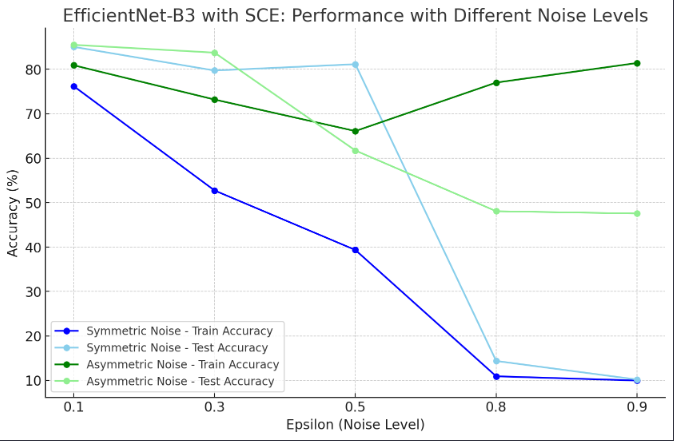
\includegraphics[width=1\linewidth, trim={0 20pt 20pt 0}, clip]{efficientnetresults.png}
    \caption{Fine-Tuned EfficientNet-B3 with SCE Loss Results}
    \label{fig:EfficientNetResults}
\end{figure}

\section{Discussion}
In this section, we discuss an unsuccessful strategy that we implemented but that provides valuable insights into the usage of unsupervised learning for this task. We'll also cover the current state-of-the-art approach and summarize the strengths of our two proposed strategies designed to handle label noise.

\subsection*{Failed Attempt: CNN-KNN Hybrid Strategy Against Label Noise}
Our initial exploration involved a hybrid CNN-KNN (Convolutional Neural Network - k-Nearest Neighbors) model, merging CNN's feature extraction with KNN's unsupervised classification capabilities \cite{sejutiHybridCNNKNN2023a}. The CNN component learned hierarchical representations through convolutional and pooling layers, and the extracted feature embeddings served as data points in a high-dimensional space. However, the model faced limitations on the noisy CIFAR-10. The success of the CNN-KNN approach relies on the separability of features, and when features between classes are too similar or overlapping, the model's performance may be hindered. This is the most probable reason behind the low performance. 

\subsection*{Current SOTA on CIFAR-10N}
Examining the current state-of-the-art in handling label noise on CIFAR-10 datasets, the Prior Guided Denoising Framework (PGDF) stands out \cite{PapersCodeCIFAR100N}. PGDF employs a two-step strategy, initially segregating samples based on training loss and then using semi-supervised methods for pseudo-label generation. Despite impressive performance gains, PGDF's extended training times and inference time did not meet the constraints of this project.

\subsection*{Applicability of the Proposed Strategies}
The SCE Loss presents a versatile solution applicable to various CNN models without significant modifications, demonstrating broad usability. Similarly, the transfer learning technique offers a straightforward way to enhance adaptability by leveraging pre-trained models. These strategies can easily complement other techniques, such as selective sampling, contributing to a robust framework for addressing label noise.


\section{Limitations}
Our strategies, ResNet18+SCE Loss and transfer learning with EfficientNet-B3+SCE Loss demonstrate limited accuracy improvement with noise levels above 50\%. Also to achieve a more optimal performance on noise levels under 50\% longer training time would be beneficial. However, practical constraints on computational resources and time limit the feasibility of extending training time.

\section{Conclusion}

In conclusion, our investigation focused on two strategies: ResNet18 with Symmetric Cross Entropy Loss (SCE Loss) and transfer learning using EfficientNet-B3 with SCE. Both strategies demonstrated improvements in test accuracy for both symmetric and asymmetric noise, achieving up to 11.71\% above the baseline for ResNet18+SCE and 14.34\% for EfficientNet-B3+SCE. Transfer learning with EfficientNet-B3 showed promise by leveraging pre-trained models to mitigate overfitting to noisy labels. However, practical constraints, including limited training time and computational resources, constrained the depth of our exploration. Despite these limitations, these strategies provide accessible alternatives and valuable insights for building robust models in the presence of label noise.



{\small
%\bibliographystyle{ieee_fullname}
\bibliographystyle{plainurl}
\bibliography{egbib}
}

\appendix
\section{Appendix}
\subsection{Additional Testing}
\begin{table}[H]
\centering
\begin{tabular}{|c|c|c|c|c|}
\hline
\textbf{\(\epsilon\)} & \multicolumn{2}{c|}{\textbf{Symmetric}} & \multicolumn{2}{c|}{\textbf{Asymmetric}} \\
\cline{2-5}
 & \textbf{Train} & \textbf{Test} & \textbf{Train} & \textbf{Test} \\
\hline
0.1 & 75.33 & 77.93 & 81.36 & 78.13 \\
\hline
0.3 & 55.28 & 74.13 & 73.10 & 75.81 \\
\hline
0.5 & 36.05 & 67.59 & 66.58 & 58.56 \\
\hline
0.8 & 11.16 & 21.61 & 77.14 & 46.75 \\
\hline
0.9 & 10.10 & 10.44 & 81.48 & 45.82 \\
\hline
\end{tabular}
\caption{Baseline Train and Test Accuracies for Symmetric and Asymmetric Noise (batch\_size = 64 and learning\_rate = 0.001).}
\label{tab:mergedAccuracyAdditional}
\end{table}

\subsection{Additional Figures}

\begin{figure}[ht]
    \centering
    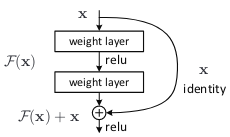
\includegraphics[width=0.7\linewidth]{resnetBlock.png}
    \caption{ResNet Block \cite{heDeepResidualLearning2015}}
    \label{fig:resnetBlock}
\end{figure}

\begin{figure}[!ht]
    \centering
    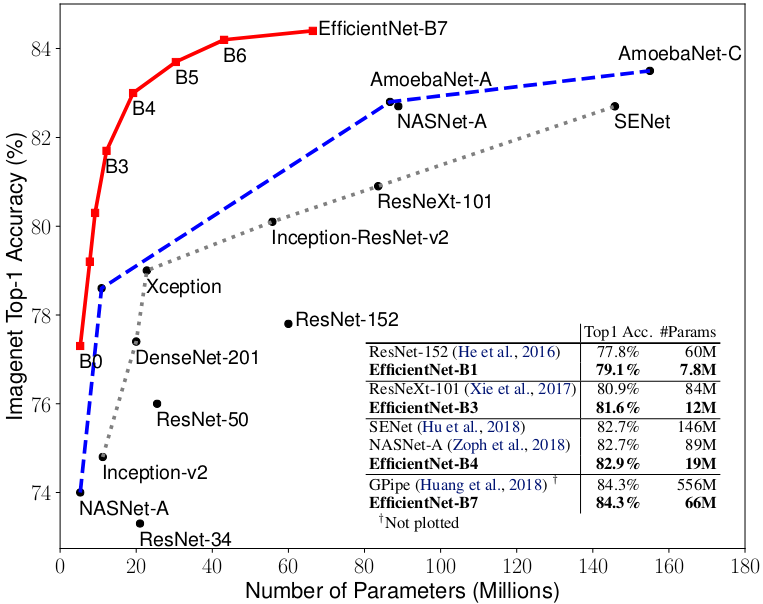
\includegraphics[width=1\linewidth]{efficientNet.png}
    \caption{Figure extracted from the EfficientNet paper \cite{tanEfficientNetRethinkingModel2020}.}
    \label{fig:efficientNet}
\end{figure}

\end{document}